\chapter{Modulation of SWR incidence}

\section{Summary}

  Sharp-wave ripples are network events in the hippocampus that involve large
  number of cells that fire in synchrony within a time window of 20-100 ms.
  Despite the huge attention that SWRs are attracting, the exact mechanisms of SW
  generation, termination are still debatable.  An in-vitro model of SWs was
  developed by Maierxxxx has largely facilited the study of the SWs. In this
  chapter I review the literature on the effects of various drugs on the SW
  incidence and discuss on the possible mechanisms of drug control on SWs.
  Moreover, I analyse 2 datasets of in-vitro recordings provided by Nikolaus and
  show that the gaabaA antagonist gabazine does not only decrease SW incidence
  but also increases SW amplitudes. GabaB antagonist SCH..., on th eother side
  increases SW incidence but decreases the amplitude of the events. The results
  suggest the existance of a limited resourse that is gettting depleted by SWs
  and recovered by time


\section{Introduction}
  general question of the origin of SWs; ca1 minislices, disinhibition, gabzine 
  a paragraph about what this chapter is about: investigate the effect of some drugs
  on SW incidence; data and theorykk
\section{Results}
%________________
  In  this section I present main results from analysing data...

  \subsection{Sharp wave peaks do not determine the interval until next event }
    \label{gabazine_invitro}

    The interval between consecutive SWR events in vitro varies from hundreds
    of milliseconds to tens of seconds depending on the experimental setup and
    slice preparation. Currently, we do not know the underlaying biological
    processes that have time scales much larger than than the time scales of
    neural activity. However, a natural assumption is that there is some kind
    of recovery of the system after each event, e.g., synaptic depletion and/or
    short-term depression \citep{Romani2015, Kohus2016}, or slower inhibition.
    Here I ask whether this recovery time depends on the size of a sharp-wave
    event, e.g., do the larger events deplete more resources, and thus, prolong
    the interval until the following event.


    To analyse the dependence between peaks and the following intervals, I used
    data provided by Nikolaus Maier. The dataset consists of extracellular
    recordings from the CA3 area of hippocampal slices which exhibit dynamics
    of spontaneous occurring sharp waves (SWs). I calculated the serial
    correlation between SW peaks and the time interval until the following
    event and found only weak correlations (Figure~\ref{fig:ca3only_SCsumm},
    left panel). From the 20 recordings, only 9 show correlations that are
    significant ($p<0.001$) with a mean correlation coefficient of around 0.2.
    The results show mostly missing or low dependence between the size of a SW
    and the interval until the following event. Moreover, the correlation
    coefficients are independent on the frequency of spontaneous events in the
    slice (Figure~\ref{fig:ca3only_SCsumm}, bottom-left panel).

    \begin{figure}
      \includegraphics[width= 35pc]{ca3only-cs2.eps}
      \caption{
        Serial correlation of spontaneous sharp waves. top-left: Distribution
        of serial correlation coefficients between sharp-wave peaks and the
        interval until the following event; only significant correlations are
        shown ($p<0.001$). bottom-left: The peak-interval correlations shown
        against the incidence for each recording. top-right: Distribution of
        interval-peak correlation coefficients and the same correlations
        plotted against incidence (bottom-right).
             }
    \label{fig:ca3only_SCsumm}
    \end{figure}

    A possible explanation for the missing peak-interval correlations is that
    the SW peaks are local phenomenon, and while being large at the recording
    location, SWs can be smaller in other locations of the slice. The next
    event is then triggered in a site where the peak has been rather low and
    the local resources are less depleted. Therefore, we can not predict the
    time of the next event based on the measured amplitude at a particular site
    as SWs can originate elsewhere in the slice, and the local depletion
    recovery does not play any role in controlling the event. Following this
    line of reasoning gives us a hypothetical explanation about the
    surprisingly low correlations between peaks and intervals.

    To test the hypothesis relying on locality of SW amplitudes stated above, I
    analysed data from multi-electrode array (MEA) recordings. The dataset was
    provided by Roberta Evangelista, where multiple sites in the CA3 area of
    hippocampal slices are measured simultaneously. In single recordings, the
    peaks of SW events measured at different locations show very high
    co-variability (an example is shown Figure~\ref{fig:peak_correlation_ex}).
    Moreover, in the aggregated data from 20 different slices show that any two
    locations in the CA3 have positive and significant ($p<0.001$) correlation
    between the measured SW peaks (Figure~\ref{fig:peak_correlation_summ}). The
    high correlations between different sites rule out the hypothesis that the
    size of SWs is a local phenomenon.

    \begin{figure}
      \includegraphics[width= 35pc]{mea.eps}
      \caption{
        An example of configuration and recording of a multi-electrode array on
        a hippocampal slice. top-left: The colored circles (red and blue)
        denote recording channels that are considered to be in the radiatum
        layer and have a reliable signal of the sharp-wave events. bottom:
        Example of a recording sweep where SW peaks measured at the recording
        electrodes are plotted in time. Here at each recording site, the peaks
        are normalized for better comparison. top-right: A matrix of the
        pair-wise correlation coefficients between SW peaks measured at the
        different electrodes.
      }
    \label{fig:peak_correlation_ex}
    \end{figure}

    \begin{figure}
      \includegraphics[width= 25pc]{mea_corrs_summ.eps}
      \caption{
              Aggregated distribution of correlation coefficients between the
              peaks of sharp waves measured at different locations in CA3 in
              hippocampal slices.
             }
    \label{fig:peak_correlation_summ}
    \end{figure}
    
    In summary, the serial correlations between events show that the amplitude
    of a SW event does not determine the time interval until next event. This
    absence of peak-interval correlations can not be explained by some locality
    of the SW events as I showed that SW peaks are non-local phenomenon, and
    large SW measured at one location is likely to be large in the whole CA3
    region. A possible explanation of this puzzling fact is proposed in the
    discussion of this chapter (is it !!!). 

  \subsection{Sharp wave sizes are determined by the interval since the last event}

    Another line of reasoning is that the duration of time passed after an SW
    events would influence the recovery of the system, e.g., after longer
    periods of time, the network has more time to recover the depleted
    resources and a larger event is to be expected. To test this idea, I
    calculated the serial correlations between the inter-event time intervals
    and the peak of the following SW (Figure~\ref{fig:ca3only_SCsumm}, right
    panel). Most of the recording show significant ($p<0.001$) and positive
    correlations (18 out of 20 recordings). This means that after a long
    interval the peak of the following SW is big, and after a brief interval,
    the following sharp wave has a smaller amplitude. 

    The high interval-peak correlations found in the data are confirmed by the
    recent results from \citep{Kohus2016}. Moreover, \citep{Kohus2016} make a
    detailed study on the inhibitory connections in the CA3 area and show that
    the synapses of parvalbumin-positive basket cells ($\rm PV^+BCs$) undergo
    short-term depression (STD) that acts on a time scale of hundreds of
    milliseconds. The authors propose that the synaptic recovery from this
    depression is responsible for the peak of SWRs observed in the local field
    potential, and moreover, suggest that this can be a possible mechanism
    controlling the incidence of SWR occurrence.
    
    Different recordings have various incidence of spontaneous SWs ranging from
    0.1 to $\sim 1 \,\rm events/sec$. A natural question is whether the
    incidence influences the serial correlations between the intervals and the
    following SW peaks. While one can speculate that there is some trend of
    positive correlation, i.e., higher incidence correlates with higher
    interval-peak correlations (Figure \ref{fig:ca3only_SCsumm}, bottom-right
    panel), this dependence is statistically insignificant (Pearson and
    Spearman tests). As the number of recordings is quite low ($n=18$) more
    data is needed to give a more precise answer to this question.
    
    In the following subsection, I extend further on this idea of how
    short-term depression of inhibitory synapses can control the incidence of
    SWRs and propose a hypothetical circuit that can explain some of the more
    contra-intuitive experimental findings on SWRs.

  \subsection{Gabazine effects on sharp-wave ripples {\textit {in vitro}} }

    Hippocampal slices exhibit network dynamics shaped by excitatory and
    inhibitory activities that balance each other. It is intuitively expected
    that by decreasing the total inhibitory coupling (connections from
    inhibitory to all the other neurons are weaken) the network would get into
    a more excitable state. However, from previous work (e.g., refs) it is
    known that application of gabazine (a $\rm GABA_A$ receptor antagonist)
    decreases the network activity and the rate of spontaneously occurring
    sharp waves. How does a decrease of inhibition lead to a more inhibited
    network. To tackle this paradox, in this section I analyse some data
    provided by Nikolaus Maier in which gabazine is applied to hippocampal
    slices.
    
    Gabazine (SR-95531) is a $\rm GABA_A$ receptor antagonist that blocks
    phasic receptors only, effectively decreasing the inhibitory conductances
    (for details, see Section \ref{sec:swr_modulation}). In the experiments
    analysed here, after a few minutes of stable baseline recording $100 \,\rm
    nM$ gabazine was applied to the hippocampal slices. A typical example is
    shown in Figure \ref{fig:gabazine_ex} where gabazine was applied 27 minutes
    after the recording onset (application duration denoted with a horizontal
    red line). Shortly after the drug infusion, the incidence of spontaneous
    events goes down while there is slight increase in the amplitude and the
    duration of the SW events. After the washout (end of red bar, at 43
    minutes) the incidence of SWs increases back to the values before the drug
    infusion.
    
    \begin{figure}
      \includegraphics[width =35pc]{6june12_slice1.png}
      \caption{
        Extracellular recording from the CA3 area where gabazine is infused the
        hippocampal slice. The time of drug application is denoted with a
        horizontal red bar. The top panel shows the SW incidence in time. The
        two panels below show the SW peaks (`fil' and `raw' stand for filtered
        and raw signal, respectively; units are mV), where the gray dots
        represent single events and the black color is the mean peak in one
        minute time step and its standard deviation. Analogously, the forth
        panel shows the SW duration in milliseconds. The panels on the bottom
        row show all events before (left) and during (middle) drug application
        overlaid in gray, and the mean wave-forms are in black. The right-most
        panel shows a comparison between the mean event before and during
        gabazine application.
      }
    \label{fig:gabazine_ex}
    \end{figure}

    Overlying all detected events (before and during drug) relatively to the
    peak of the filtered signal and calculating their mean value shows a
    stereotypical SW waveform (Figure~\ref{fig:gabazine_ex}, bottom panels).
    Here, the mean sharp wave is larger after the drug injection (bottom-right
    panel). It is worth noting that in this example recording, there is some
    high-frequency noise in the measured LFP (peaks of the gray traces), likely
    reflecting the spiking of one or more neurons located nearby the recording
    electrode. In this example, the network activity seems to be less noisy
    after the application of gabazine.

    Gabazine decreased the incidence in all 8 recordings. The average
    effect is shown in Figure~\ref{fig:gabazine_sum} where the incidence is
    normalized relative to the incidence before drug application. Gabazine
    starts affecting the incidence already 1 minute after application and takes
    around 5 minutes to take a full effect. 
    
    \begin{figure}
      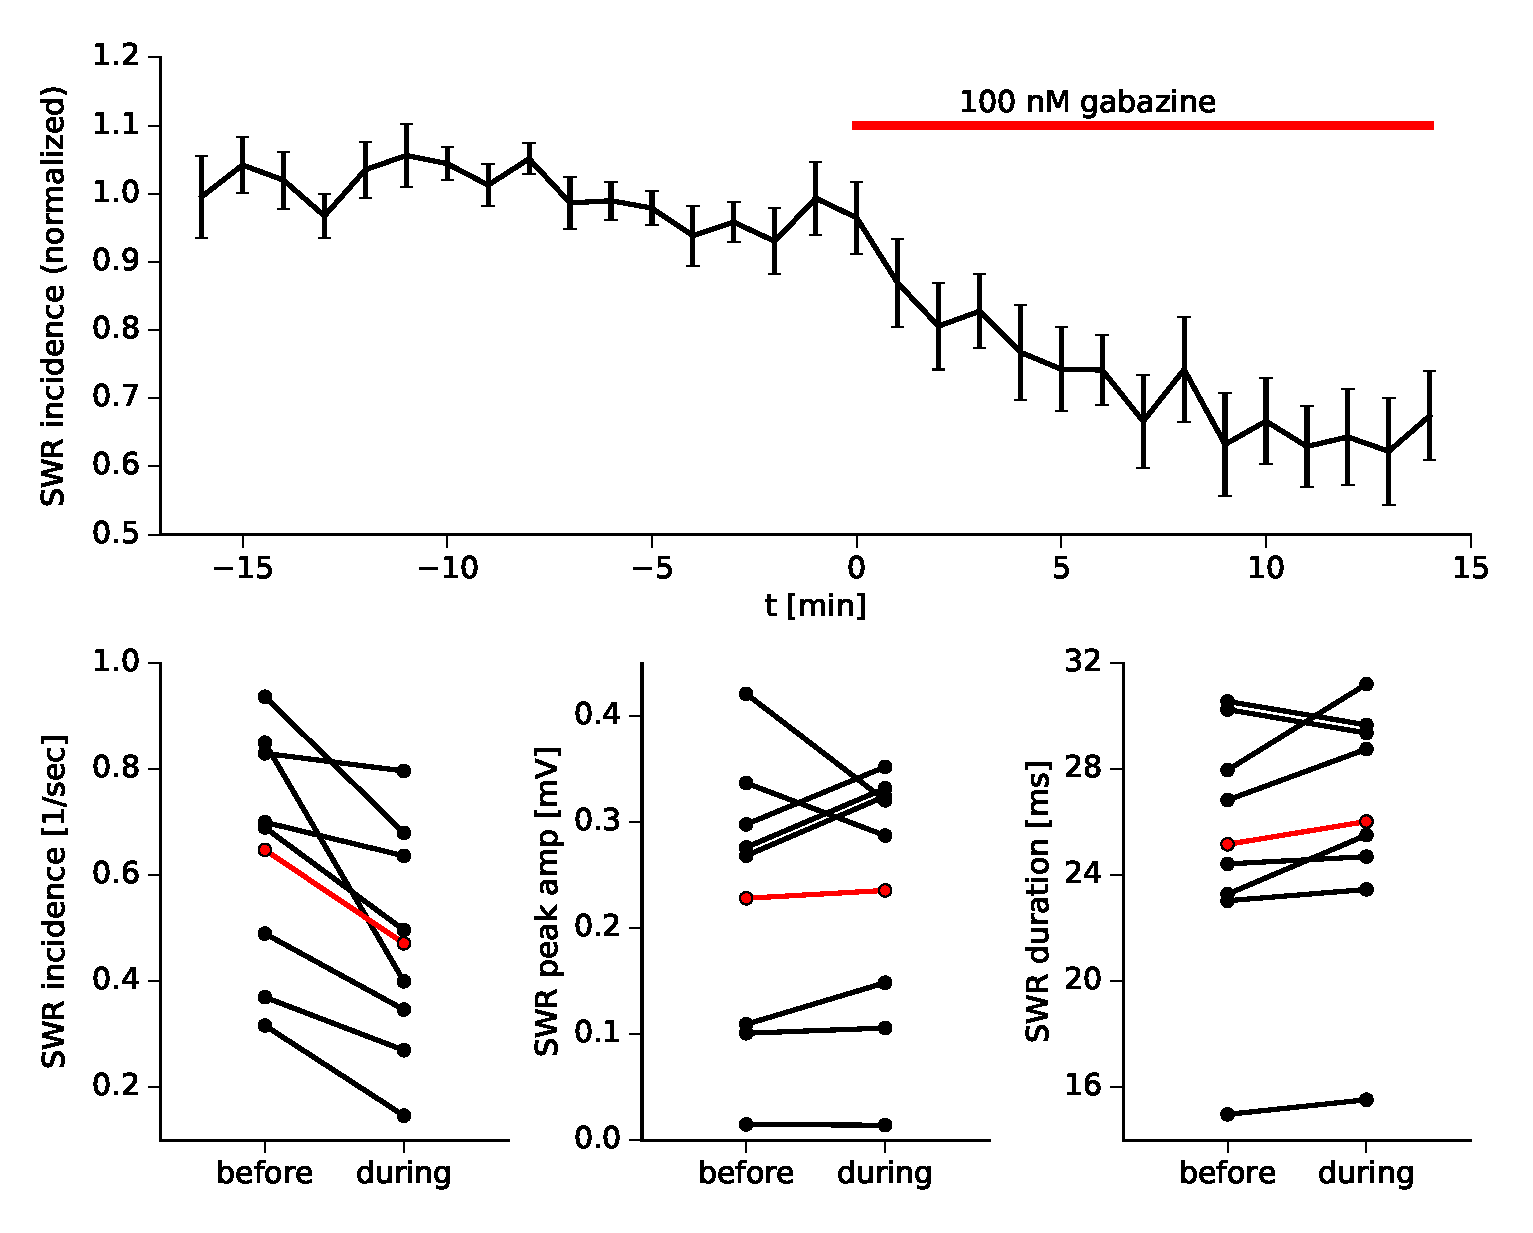
\includegraphics[width =35pc]{gabazine_events_all.eps}
      \caption{
        Gabazine effects on sharp waves. top: SW incidence in time aggregated
        from all recordings ($n=8$), where the incidence before the drug
        application is normalized to 1. bottom: SW incidence, peak and duration
        measured in 5-minutes time windows before and during gabazine
        application.
      }
      \label{fig:gabazine_sum}
    \end{figure}

    To better characterize how the drug affects the network dynamics, further,
    the analysis focuses on the events in constrained time windows only. Events
    from the window [-7, -2] minutes (before drug application) and [6, 11]
    minutes (after drug application) were used to calculate properties of SWs
    (Figure~\ref{fig:gabazine_sum} bottom row). As already mentioned, there is a
    strong effect on the incidence. However, somewhat weaker effects are
    observed on the SW peak and duration. Events tend to get bigger after
    gabazine application, i.e., to have larger peak (5 out of 8 recordings) and
    to last longer (6 out of 8). 

    The found effects on the event size are in odds with the finding of
    \citep{Schlingloff2014} who showed that a local puff of gabazine \textit{in
    vitro} decreases the SWR amplitude around the application site. A possible
    explanation is that the incidence in \citep{Schlingloff2014} is intact as
    SWRs occur at other locations of the slice unaffected by the drug. The
    puffed location, however, needs more time to recover from previous events
    and, therefore, the frequent events occurring elsewhere can not engage
    fully the affected subnetwork. In the slices used in our analysis, however,
    the gabazine infusion is global which results in slight increase of the SWR
    peaks and also a decrease of incidence.
    
    \begin{figure}
      \includegraphics[width =35pc]{Schlingloff_3bcd5e.png}
      \caption{local application of Gabazine decreases amplitude, spikes (b,c,
        and d from their Fig3), increases PVBC firing (e from their Fig 5)
            }
    \label{fig:schlingloff_gabazine}
    \end{figure}

    Does gabazine have any effect on the serial correlation between consecutive
    events? To answer this question, the serial correlations (peak-interval and
    interval-peak) were measured before and after drug application in 5 minutes
    time windows as described above (Figure~\ref{fig:gabazine_SCsumm}). While
    the peak-interval correlations remain low and do not change after the
    gabazine application, there is a trend of increase in the interval-peak
    correlations. Showing the relation between incidence and interval-peak
    correlations for individual recording (Figure~\ref{fig:gabazine_SCsumm})
    reveals the tendency of decreasing incidence and increased interval-peak
    correlations (6 out of 8 recordings).

    \begin{figure}
      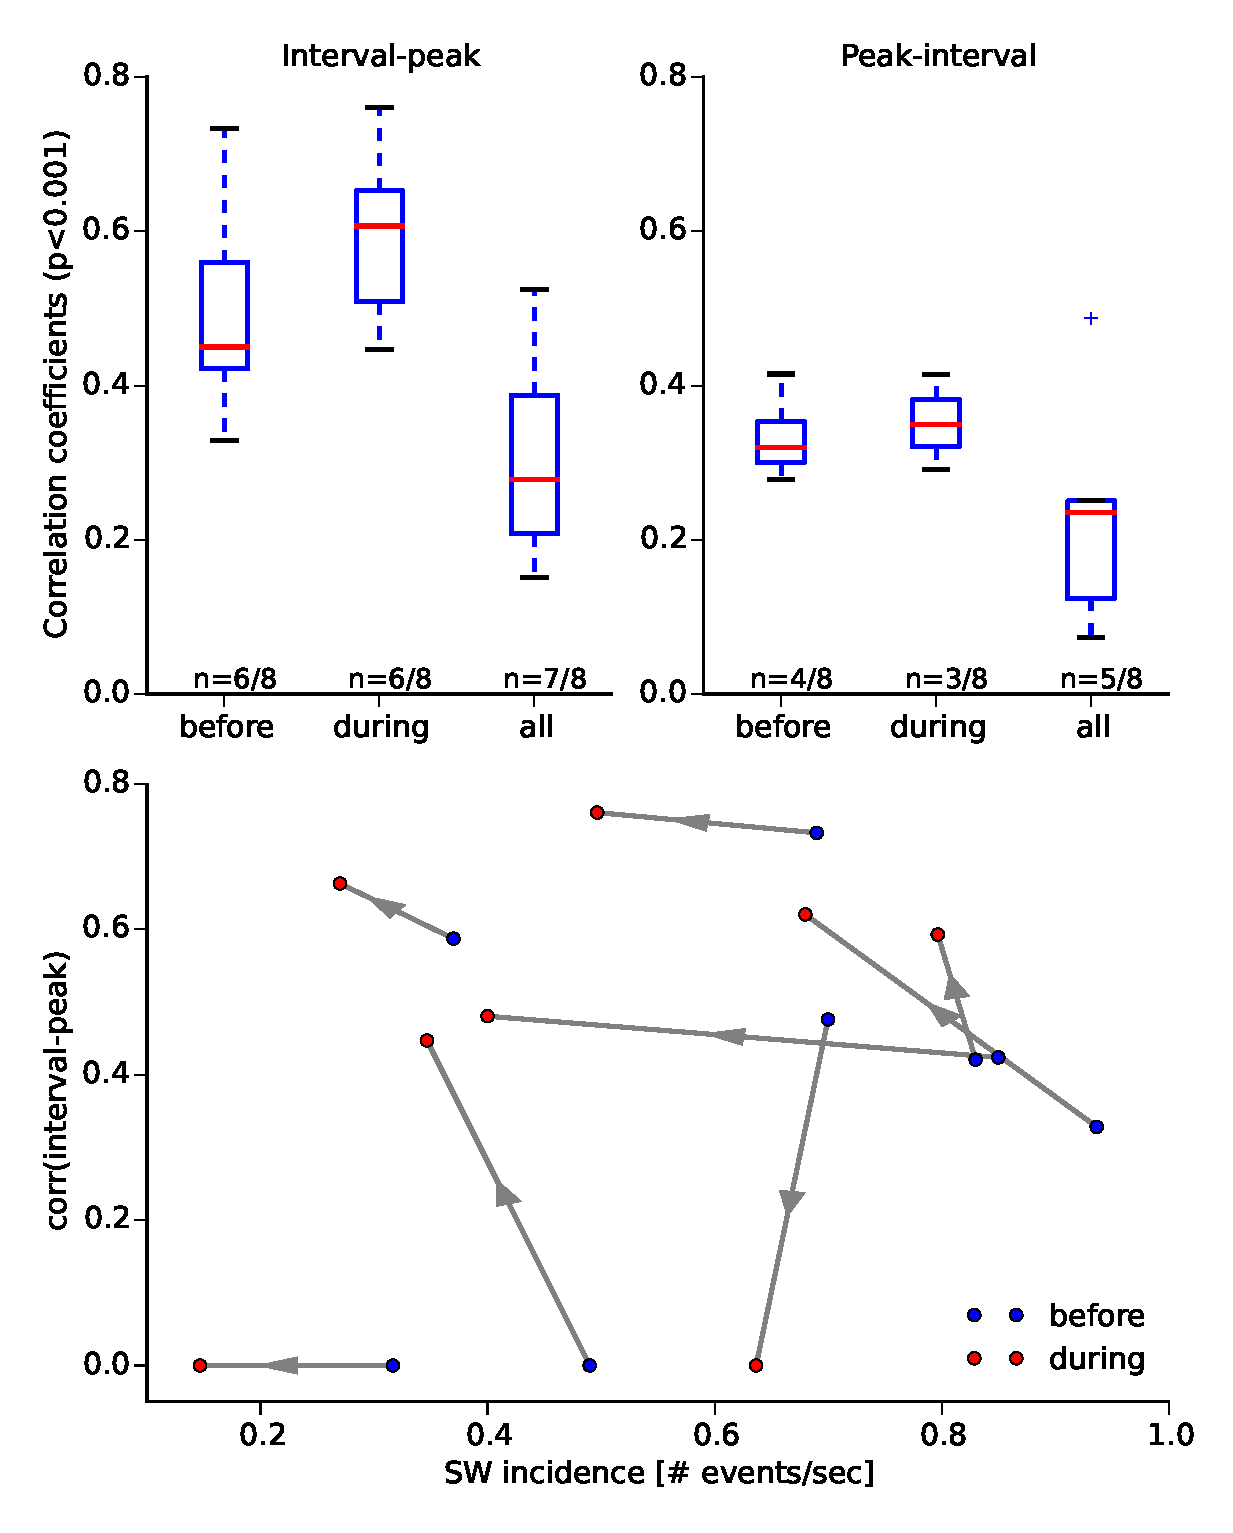
\includegraphics[width= 30pc]{gabazine_SCsumm.eps}
      \caption{
        Gabazine effect on the serial correlations. top: Serial correlation
        before and during gabazine are calculated in 5-minutes long time
        windows, where $n$ shown the number of recordings that showed
        significant correlations ($p<0.001$). bottom: Serial correlations
        coefficients between interval and the following SW peak are plotted
        against recorded incidence; arrows show the change after gabazine
        application.
             }
    \label{fig:gabazine_SCsumm}
    \end{figure}

    In summary, gabazine has the contra-intuitive effect of decreasing the
    incidence of SWRs. Moreover, gabazine application has weak effects in
    increasing the SWR amplitudes and the serial correlations between
    inter-sharp-wave interval and the peak of the consecutive SWR. However, due
    to the small dataset (8 recordings), I can not present a conclusive
    evidence of the drug effects.

  \subsection{Gabazine influence on SWR incidence {\textit {in silico} }}

    To better understand how does gabazine affect the incidence of SWRs
    {\textit {in silico}}, I deploy the assembly-sequence concept (described in
    Chapter~\ref{chap:memoryreplay}) as a model for the spontaneously occurring
    SWs. Here, numerical simulations of balanced networks with embedded assembly
    sequences and a linear firing rate model are used as tools to describe the
    network dynamics under the influence of gabazine.
      
    In the numerical simulations, sequences of neural assemblies consisting of
    both excitatory and inhibitory neurons are embedded into a randomly
    connected network. Recurrent connectivity ($p_{\rm rc}=0.08$) describes the
    connection probability within an assembly while a feedforward connectivity
    ($p_{\rm ff}=0.06$) is the connectivity between the excitatory neurons of
    consequent assemblies in the sequence (sketch of network connectivity is
    shown in Figure~\ref{fig:net_sketch}). With these parameters values, noise
    fluctuations in the firing rates get amplified by the feedforward structure
    resulting in spontaneous replays (Figure~\ref{fig:spontan}). For a more
    detailed description of the numerical model and the parameter values,
    please refer to Chapter~\ref{chap:memoryreplay}. Here, the effects of
    gabazine are modeled simply by decreasing the conductances of the targeted
    inhibitory synapses with a fixed rate (i.e., $10\%$).

    Not surprisingly, gabazine drastically increased the rate of spontaneous
    replays of assembly sequences in the modelled network. This is illustrated
    in Figure~\ref{gabzine_sim}, where gabazine is applied to all inhibitory
    synapses after the $21^{\rm st}$~second of the simulation. The top two
    panel show raster plots of the excitatory and inhibitory neurons where the
    black dots show individual spikes, and the black stripes are burst of
    synchronous activity during which many neurons fire in close temporal
    proximity. The replays during these activity bursts are used as a model of
    the sharp-wave events. The frequency of these population events is
    increased immediately after the gabazine infusion, as seen in the number of
    replays (the top panel), and in the firing rates (third panel). This result
    is in direct collision with the gabazine effects that are reported
    {\textit{in-vitro}} (Section~\ref{gabazine_invitro}).

    \begin{figure}
      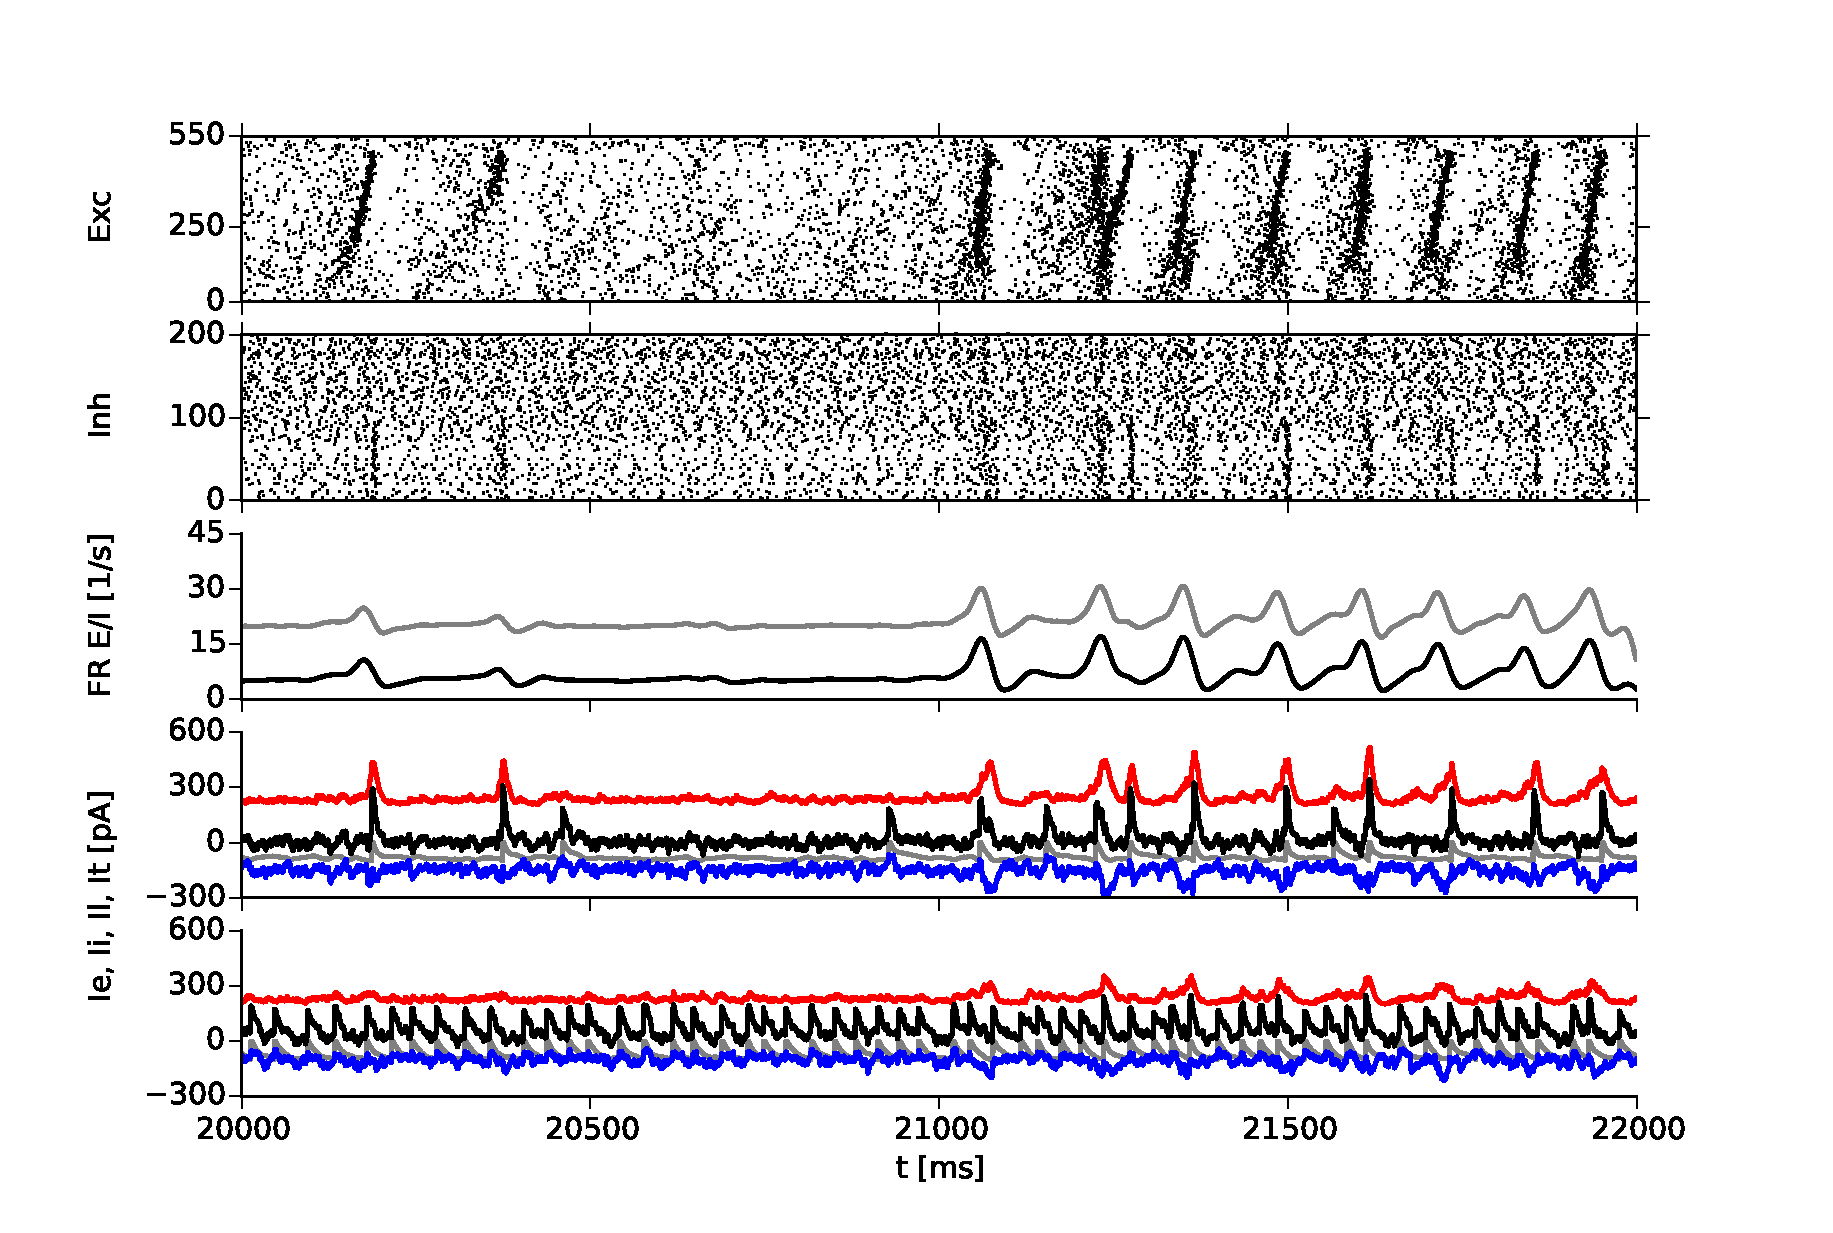
\includegraphics[width =35pc]{gabazine_sim.eps}
      \caption{Decreasing all inhibitory conductances leads to increase in
        spontaneous replays in balanced-network simulations.
            }
    \label{fig:gabazine_sim}
    \end{figure}

    Can a relatively simple two-populations balanced network explain the
    gabazine-associated decrease of SWR incidence reported in experiments?
    $\rm GABA_A$ receptors ($\rm GABA_A R$) are known to be complex channels
    with six subunits that can come in various combinations (for the curious
    readers, see Section~\ref{sec:gabaa_intro}). The expressed subunits largely
    determine the receptor properties, i.e., time constants, affinity to GABA
    and other neurotransmitters. For example tonic $\rm GABA_A R$ are
    insensitive for gabazine at low concentrations while phasic $\rm GABA_A R$
    show various affinity depending on the subunit expression. The subunit
    expression is largely determined by the type of the postsynaptic neuron and
    of the location that the channels are located on the morphological tree
    \ref{???}. One hypothesis to explain the gabazine-associated decrease of SW
    events relies on the assumption that gabazine has differential effect on
    the different $\rm GABA_A$ synapses. And more specifically, if
    inhibitory-to-inhibitory synapses are affected to a larger degree than the
    inhibitory-to-excitatory synapses, one would expect a network that is less
    disinhibited, and thus, the excitatory population receives more inhibition
    resulting in smaller firing rates. In what follows, I test whether such
    assumptions would really decrease the incidence of modeled events.

    As a toy example in numerical simulation, I consider the extreme case where
    gabazine affects the inhibitory-to-inhibitory synapses only. As expected,
    the firing rate of the excitatory neurons is decreased
    (Figure~\ref{fig:gabazine_sim_giionly}). However, the network shows a
    decrease in the firing rate of the inhibitory population as well. How is it
    possible that excitatory neurons receiving weaker inhibition (smaller input
    rate), fire less? To better understand the effects of gabazine, further, I
    present an analytical approach.
    
    \begin{figure}
      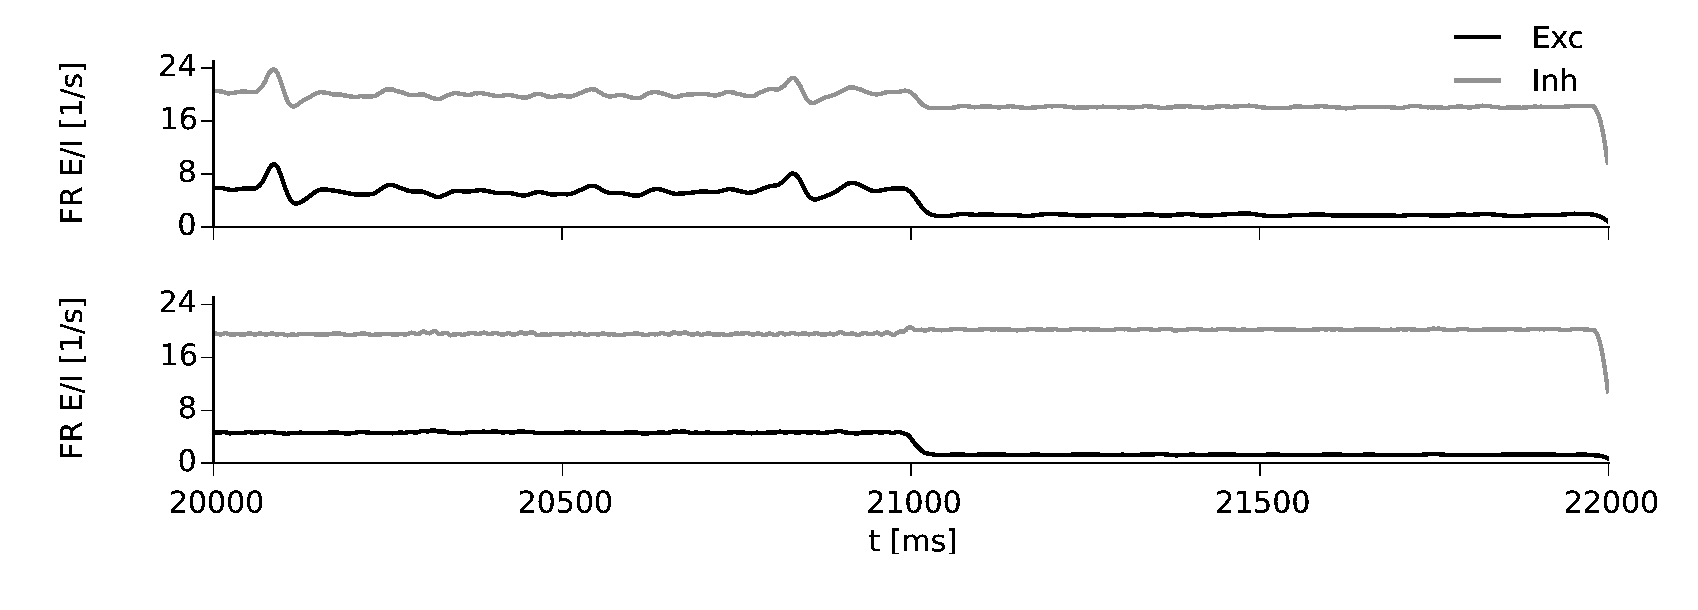
\includegraphics[width =35pc]{gabazine_sim_gii.eps}
      \caption{Decreasing inhibitory-to-inhibitory conductances only leads to a decrease of both excitatory and
                inhibitory firing rates and of spontaneous replays as well...
      }
    \label{fig:gabazine_sim_giionly}
    \end{figure}

    To capture the network dynamics, I apply a linear model of a two-population
    balanced network and analyse how the rates depend on gabazine. The network
    dynamics is described by the system of differential equations:
    \begin{equation}
      \begin{split}
        \tau \frac{\text{d}r^E}{\text{d}t} &= - r^E + w_{\rm ee} \, r^E -w_{\rm ei} \, r^I + I_0\\
        \tau \frac{\text{d}r^I}{\text{d}t} &= - r^I + w_{\rm ie} \, r^E -w_{\rm ii} \, r^I + I_0\\
      \end{split}
      \label{eq:balanced_net}
    \end{equation}
    where $r^E$ and $r^I$ are excitatory and the inhibitory firing rate,
    respectively. The connection from population $x$ to $y$ is described by the
    connection weight $w_{\rm yx}$ ($x,y = e, i$). The population time constant
    is $\tau$, and the external input to the populations is denoted with $I_0$.

    Assuming that the network is in a steady state, then the rates are
    constant, i.e., $ \frac{\text{d}r^E}{\text{d}t} = 0$ and
    $\frac{\text{d}r^I}{\text{d}t} = 0 $. In this condition, one can express
    the stationary solution:
    \begin{equation}
      \begin{split}
        r^E &= \frac{(1+w_{\rm ii} - w_{\rm ei})}{w_{\rm ie}w_{\rm ei} -
                (1+w_{\rm ii})(-1+w_{\rm ee})} I_0 \\
        r^I &= \frac{(1+w_{\rm ie} - w_{\rm ee})}{w_{\rm ie}w_{\rm ei} -
                (1+w_{\rm ii})(-1+w_{\rm ee})} I_0
      \end{split}
      \label{eq:balanced_sol}
    \end{equation}
  
    To estimate how gabazine-induced decrease of inhibitory connections
    affects the firing rates, we can look at the derivatives of the
    steady-state rates in respect to the gabazine concentration $c_{\rm gbz}$:
    \begin{equation}
      \frac{\partial r^E}{\partial g_{\rm gbz}} =
      \frac{\partial r^E}{\partial w_{\rm ei}} \cdot \frac{\partial w_{\rm ei}}{\partial g_{\rm gbz}} + 
      \frac{\partial r^E}{\partial w_{\rm ii}} \cdot \frac{\partial w_{\rm ii}}{\partial g_{\rm gbz}}
      \label{eq:re_chain}
    \end{equation}
    and
    \begin{equation}
      \frac{\partial r^I}{\partial g_{\rm gbz}} =
      \frac{\partial r^I}{\partial w_{\rm ei}} \cdot \frac{\partial w_{\rm ei}}{\partial g_{\rm gbz}} + 
      \frac{\partial r^I}{\partial w_{\rm ii}} \cdot \frac{\partial w_{\rm ii}}{\partial g_{\rm gbz}}.
      \label{eq:ri_chain}
    \end{equation}

    The partial derivatives of the rates in respect to the inhibitory weights
    can easily be estimated from Equation~\ref{eq:balanced_sol}:
    \begin{equation}
      \begin{split}
        \frac{\partial r^E}{\partial w_{\rm ii}} &= 
              I_0 \frac{w_{\rm ei} (1 + w_{\rm ie} - w_{\rm ee})} {D^2} \\
        \frac{\partial r^I}{\partial w_{\rm ii}} &=
              I_0 \frac{(-1 + w_{\rm ee})(1 + w_{\rm ie} - w_{\rm ee})} {D^2} \\
      \end{split}
      \label{eq:drdwii}
    \end{equation}

    \begin{equation}
      \begin{split}
        \frac{\partial r^E}{\partial w_{\rm ei}} &=
              I_0 \frac{-(1 + w_{\rm ii}) (1 + w_{\rm ie} - w_{\rm ee})} {D^2} \\
        \frac{\partial r^I}{\partial w_{\rm ei}} &=
              I_0 \frac{-w_{\rm ie} (1 + w_{\rm ie} - w_{\rm ee})} {D^2} \\
      \end{split}
      \label{eq:drdwei}
    \end{equation}
    where $D=w_{\rm ie}w_{\rm ei} - (1+w_{\rm ii})(-1+w_{\rm ee})$.
    
    If we now assume that gabazine has the same effect on all inhibitory
    synapses, i.e., $\frac{\partial w_{\rm ei}}{\partial g_{\rm gbz}} =
    \frac{\partial w_{\rm ii}}{\partial g_{\rm gbz}}$, the rate to gabazine
    dependence is:
    \[
      \frac{\partial r^E}{\partial g_{\rm gbz}} =
            \frac{\partial w_{\rm ii}}{\partial g_{\rm gbz}} \cdot
            I_0 \frac{-(1 + w_{\rm ii} - w_{\rm ei}) (1 + w_{\rm ie} - w_{\rm ee})} {D^2} =
            - \frac{\partial w_{\rm ii}}{\partial g_{\rm gbz}} \cdot \frac{r^E r^I}{I_0}
    \]

    \[
      \frac{\partial r^I}{\partial g_{\rm gbz}} =
            \frac{\partial w_{\rm ii}}{\partial g_{\rm gbz}} \cdot
            I_0 \frac{- (1 + w_{\rm ie} - w_{\rm ee})^2} {D^2} =
            - \frac{\partial w_{\rm ii}}{\partial g_{\rm gbz}} \cdot \frac{r^I r^I}{I_0}
    \]
    It is easy to see that the derivatives above are always positive (as
    $\frac{\partial w_{\rm ii}}{\partial g_{\rm gbz}} < 0 $), i.e., gabazine
    will always increase the rate of both excitatory and inhibitory
    populations. 

    Can this linear model model explain that in simulations in which gabazine
    affected only inhibitory-to-inhibitory synapses there was decrease not only
    in the excitatory but also in the inhibitory firing rate? Taking the rate
    derivatives in respect to $w_{\rm ii}$ only (In Equations~\ref{eq:re_chain}
    and \ref{eq:ri_chain}, we assume that $\frac{\partial w_{\rm ei}}{\partial
    g_{\rm gbz}} = 0$), it is easy to see that $\frac{\partial r^E}{\partial
    g_{\rm gbz}} < 0 $ meaning that excitatory rate will always increase when
    only $w_{\rm ii}$ is depressed. On the other hand, $r^I$ shows more
    interesting behaviour that depends on the excitatory-to-excitatory weights.
    For intermediate values $w_{\rm ee} \in (1, 1+w_{\rm ie})$, the inhibitory
    rate decreases as well during gabazine application (as seen in
    Figure~\ref{fig:gabazine_sim_giionly}). For values of $w_{\rm ee}$ outside
    of this interval, one would expect increase of inhibitory firing after the
    drug infusion. To test again whether low/high wee increases ri!!!!
    %I tested that by using lower (5 times smaller than default)
    %and higher (5 times larger than default) excitatory-to-excitatory
    %connectivity in the numerical model and found that inhibitory rate is
    %indeed increased (not shown here).

    To summarize the results from this section, by using numerical simulations
    and linear analytical description, I showed that in a balanced network
    gabazine is increasing the firing rates of both inhibitory and excitatory
    populations. This increase of firing leads to higher incidence of
    sponatenous replays which is in odds with counterintuitive decrease of
    incidence observed {\textit {in vitro}}. Therefore, I tested whether a
    differential effect of gabazine on different synapses can explain the
    experimental results. I considered the extreme case when gabazine affects
    only inhibitory-to-inhibitory synapses and showed that in this case we can
    always expect decrease in the rate of excitatory population. This result
    suggest that possibly stronger effects of gabazine on the inhibitory
    neurons might explain the decreased SWR incidence after gabazine
    application {\textit {in vitro}}.
    
  \subsection{The role of $\rm GABA_B$ receptors}

    SWs are huge population events where many PC and interneurons are firing
    with increased FRs, which is especially pronounced for the perisomatic
    targeting PVBCs and axo-axonic cells? \ref{kalusberger?}.  It has been
    shown that the repetitive firing of interneurons can activate extrasynaptic
    $\rm GABA_B$ receptors possibly through increased concentrations of ambient
    GABA in the extracellular space \ref{???}. The inhibition from $\rm GABA_B
    Rs$ is relatively slow lasting several hundreds of milliseconds, which is
    close to the time scale of the typical inter-SW intervals. Here, I study
    the possibility the relatively long time intervals between SW events are
    determined by $\rm GABA_B Rs$.
    
    First, to investigate whether $\rm GABA_B$ is involved in the SW incidence
    in the {\textit{in-vitro}} model, I analysed extracellular recordings where
    $\rm GABA_B R$ antagonist SCH50,911 was applied to the slice. The number of
    recording is 13, but here I excluded one recording as it exhibits virtually
    no events prior to the drug application, and thus, heavily skews the average
    results. The drug effects are reflected in the network dynamics quite fast,
    as the incidence of SWs increases already during the first minute of
    application (see the example recording in Figure~\ref{fig:gB_example}, top
    panel). The main properties of the SWs are stable during the whole
    recording, and there is only a slight decrease in amplitudes shortly
    after the drug application.
    
    \begin{figure}
      %\includegraphics[width =35pc]{19march13_slice1.png}
      \includegraphics[width =35pc]{21sept_slice3.png}
      \caption{ 
        Example recording. GabaB antagonist increases SWR incidence 
              }
    \label{fig:gB_example}
    \end{figure}

    Blocking the $\rm GABA_B Rs$ resulted in increased incidence of spontaneous
    sharp waves in the aggregated data from all recordings. The drug effects
    are visible already in the first minute after the application and saturate
    around 2-3 minutes later (Figure~\ref{gB_summ}, top panel). To better
    assess the effects of SCH further, the analysis focuses on the events in
    5-minutes long time windows, i.e., in the intervals [-5, 0] and [2, 7]
    minutes, for before and during drug application, respectively. Comparing
    the incidence in these two intervals shows that SCH increases the incidence
    in every recording, and there is a tendency of decreased peak (9 out of 12)
    and duration (10 out of 12) of sharp waves (Figure~\ref{gB_summ}, bottom
    panels). While the result for every recording varies depending on the exact
    time window that is used for the analysis, the summary result does not
    change qualitatively.
    
    \begin{figure}
      \includegraphics[width =35pc]{SCH_all.eps}
      \caption{GB antagonist pooled
              Bottom: mean values before the drug is infused (from -5 to 0 mins), and after (from 2-7 mins)
            }
    \label{gB_summ}
    \end{figure}

    Next, I inquire whether blocking $\rm GABA_B Rs$ affects also the serial
    correlation between events. At first glance the pooled data does not reveal
    any change in the correlations distribution (Figure~\ref{gB_SCsumm}, top
    panels).  However, looking at effects in the individual recordings
    (Figure~\ref{gB_SCsumm}, top panels) one can see that there is a clear
    trend in the decrease of serial correlation after drug application (10 out
    of 12 recordings, 2 recordings show no significant correlations).

    \begin{figure}
      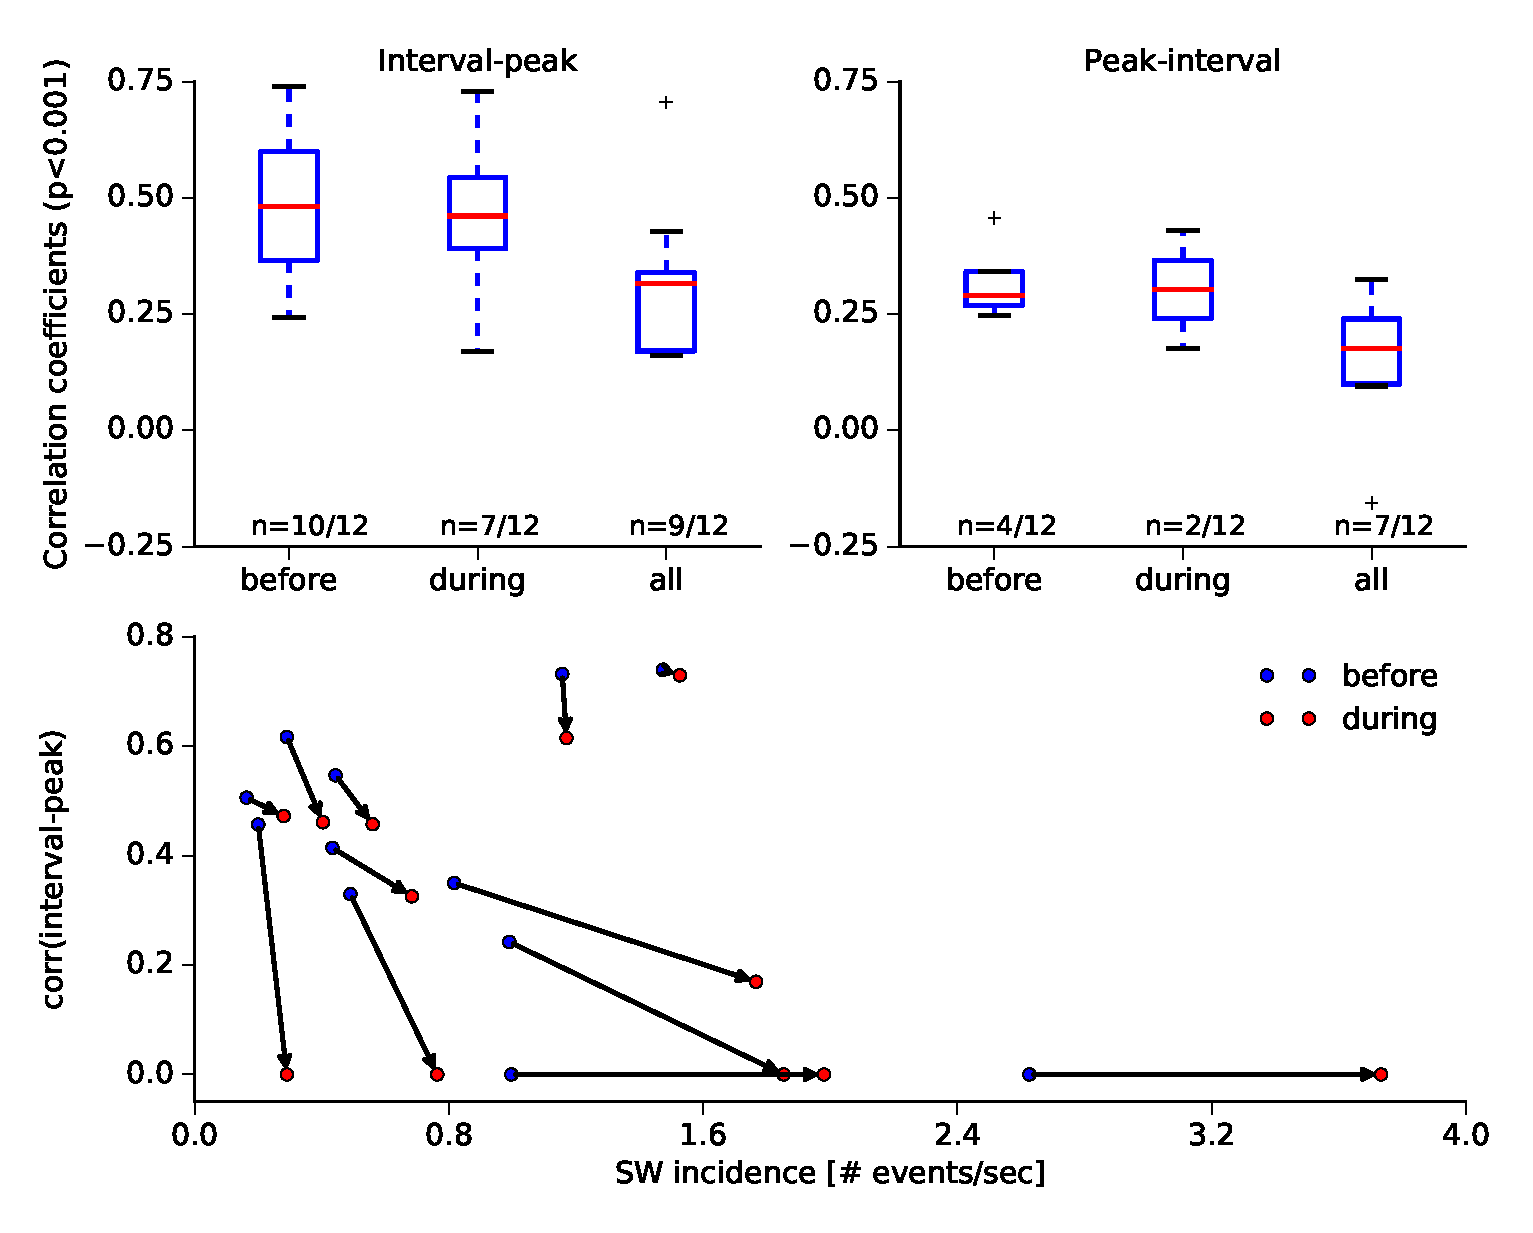
\includegraphics[width =35pc]{SCH_SCsumm.eps}
      \caption{GB SC
            }
    \label{gB_SCsumm}
    \end{figure}

    To summarize the above findings, GBRs are taking part in the SW modulation
    by increasing incidence and decreasing peak and duration. However, the
    increase is on average less than two-fold suggesting that $\rm GABA_B$ is
    not the only mechanism with a slow time constant controlling the incidence.
    Moreover, blocking $\rm GABA_B Rs$ leads to a decrease in the serial
    correlations between interval and peaks, Which is puzzling given the
    increased incidence.  To investiagate how does $\rm GABA_B Rs$ influence
    the SW incidence it is worth having a closer look at the possible
    involvement of the different $\rm GABA_B$ channels.

    % up to here corrected on paper!
    It is been shown that a repetitive firing of certain interneurons can evoke
    strong and slow inhibition due to activation of GBRs on pyramids
    \ref{blabla}. As SWs are population events that recruit many neurons, and
    especially the perisomatic targeting INs \ref{Klausberg??}, it is likely
    that ambient gaba in this region is increased. Next I ask whether GBRs
    located postsynaptically on the PC are indeed activated after SWs and
    whether they play any role in the modulation of SWs. To test this
    hypothesis, here I analyse data from simultaneous extracellular and
    intracellular recordings performed in the radiatum layer of the hippocampal
    CA3 area and a pyramidal cell in the CA3, respectively. By averaging the
    intracellular traces across events, we can see that a GB hyperpolarization
    is present in a few recordings, but is not is not visible in the mean of
    all recordings (Figure \ref{fig:intra_means}, top panel). Most
    intracellular traces show various combination of depolarization and
    hyperpolarization, indicating a rich dynamics of excitatory and inhibitory
    inputs. In the recordings that show a slow hyperpolarization (4 out of 13
    recordings, shown in Figure \ref{fig:intra_means}, bottom panel) the trough
    in the membrane potential is around $200 \, \rm ms$ after the population
    event and lasts for about $500 \, \rm ms$. Interestingly, only one
    recording reveals well-pronounced slow as well as fast inhibition (red
    trace).

   \begin{figure}
      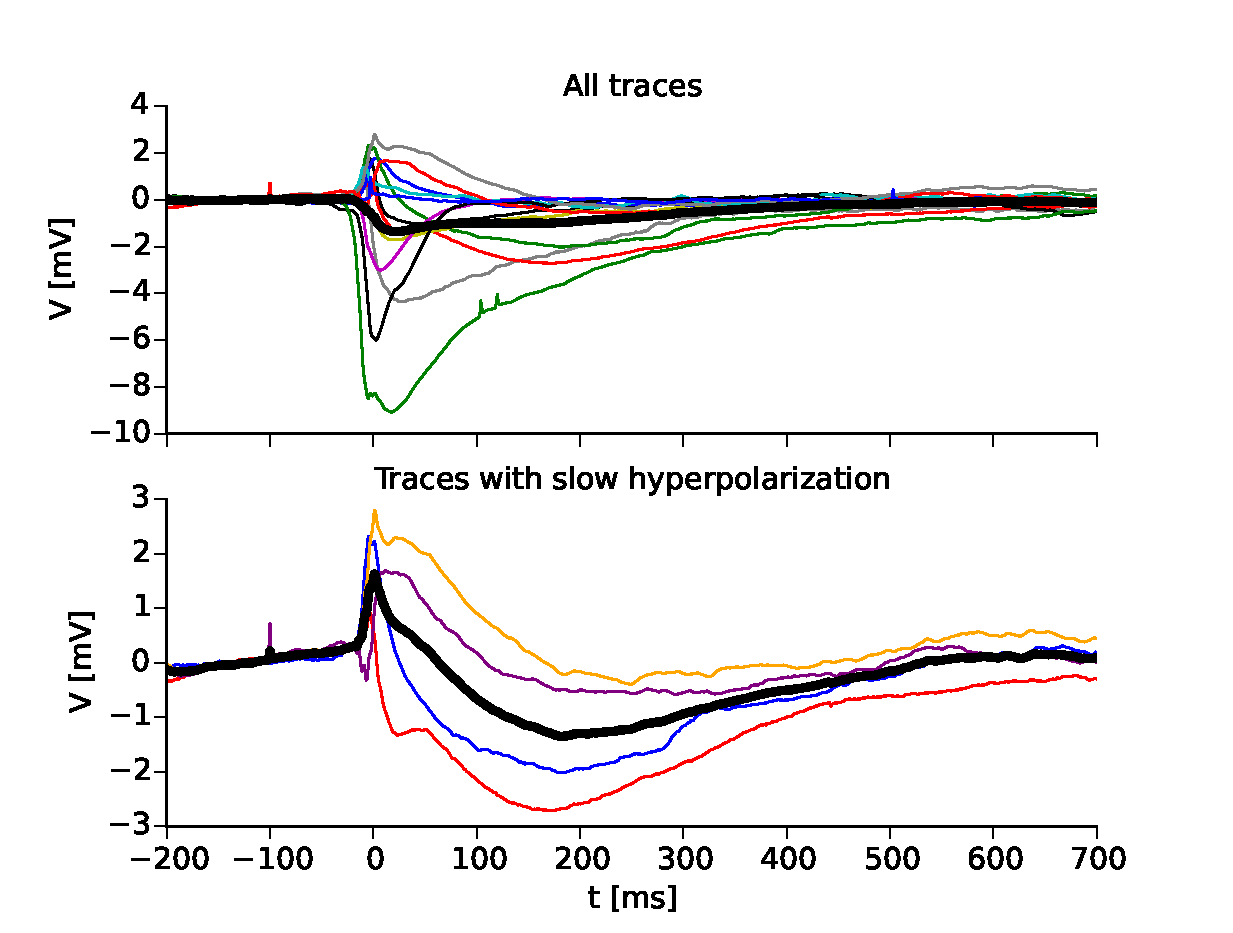
\includegraphics[width =30pc]{mean_intras.eps}
      \caption{ Mean SW-associated voltage traces for the different cells are color coded;
        the thick black line is the mean of the means. bottom: mean voltage traces of
        cells that show slow, possibly gB-evoked hyperpolarization. all
        traces are normalized by subtracting the mean potential the before
        the event.
              }
      \label{fig:intra_means}
    \end{figure}

    gB polarisation is correlated with the size of events
    gB response is not correlated with the interval till next event, which is an evidence against the hypothesis proposed above

    Is the slow hyperpolarization correlated in any way with the amplitude of
    the SWs? To test this, I separated the events in each recording in two
    groups: big and small events, for events that from the 30\% biggest or 30\%
    smallest events, respectively. Plotting the mean intracellular trace during
    small and big events, shows that the SWs with larger amplitudes are
    associated with larger hyperpolarization (Figure~\ref{fig:intra_big_small},
    top panel). Interestingly, the mean traces before big and small events are
    virtually indistinguishable (Figure~\ref{fig:intra_big_small}, bottom
    panel), suggesting that the hyperpolarization does not determine the size
    of the following event. This result holds for the four recordings that
    exhibit slow inhibition in the voltage potential. Moreover, testing whether
    the slow hyperpolarization affects the interval until the following events
    also gave negative results.

    \begin{figure}
      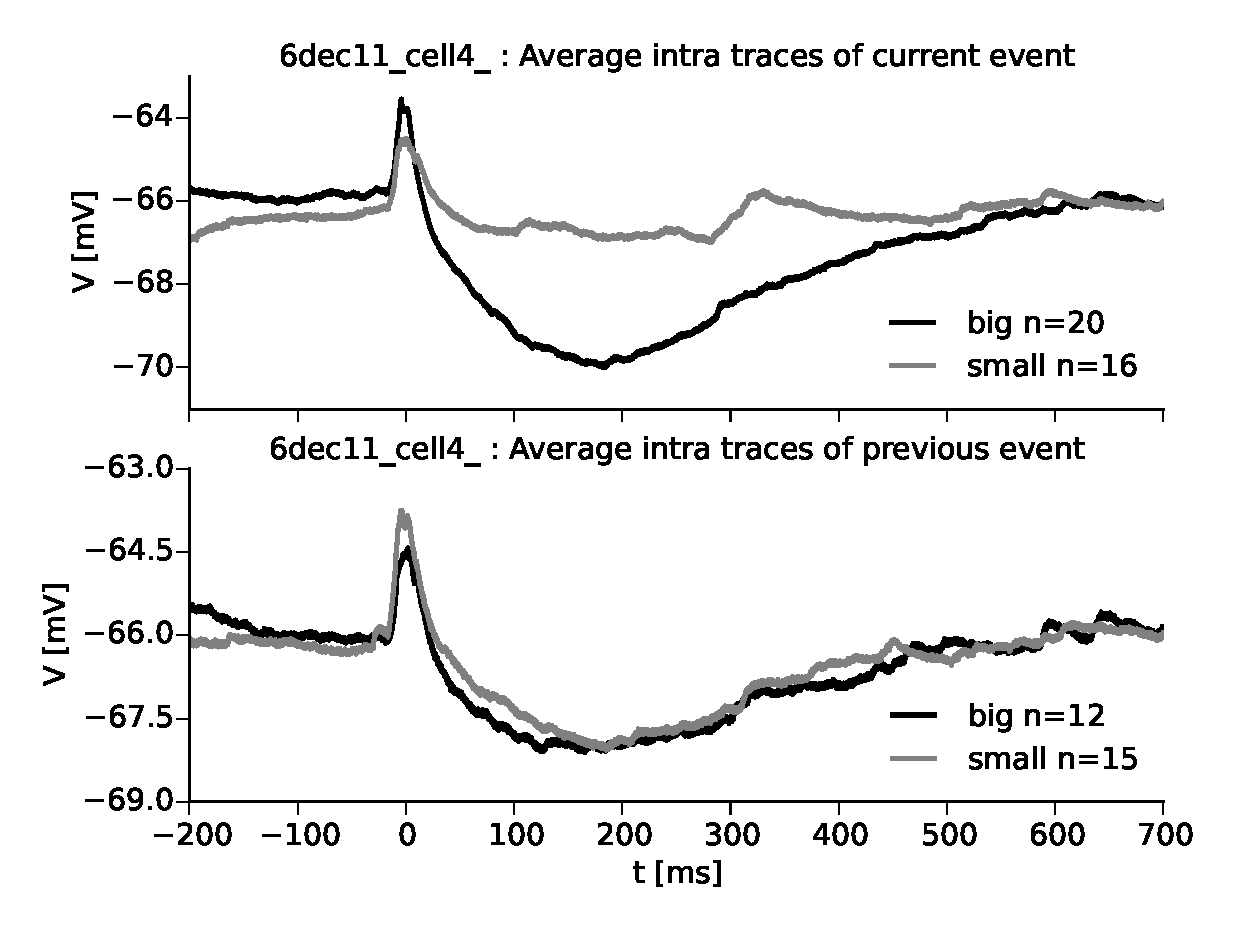
\includegraphics[width =30pc]{6dec11_cell4_000.eps}
      \caption{ Example recording. Big events are associated with a larger
        hyperpolarization (top). Here smaller events (30\% of the smallest
        SWs) did not evoke gB-associated response. Bottom: there is no
        correlation between the depolarisation of a cell and the size of the
        following event.
              }
    \end{figure}

    The last dataset of intracellular and extracellular recordings reveals that
    slow, possibly $\rm GABA_B$-associated hyperpolarization occurs only in
    fraction of the CA3 pyramidal neurons {\textit{in vitro}}. The magnitude of
    the received inhibition is not correlated with the size or the time
    interval until the next event. Therefore, I conclude that postsynaptic $\rm
    GABA_B$ receptors do not play a central role in controlling the rate of
    sharp-wave ripples.
 
    However, seems not to be crucial for SWRs, but only facilitates a bit?

    In summary, the gB antagonist SCH lead to increase in SW incidence in the in SW vitro model analysed here....?

    presynaptic effects of gB; likely not due to postsynaptic gBR on PY neurons (from simultaneous intra/extra recordings dataset); Maier2012? also suggests presynaptic effects of gB; however
      
    SCH decreases peak
      
    decreased peak means decreased currents; however, blocking presynaptic gBR would lead to increased single IPSC/P; therefore likely that SCH decreases FR of perisomatic targeting INs during SW events

\section{Discussion}
  \subsection{Hypothesis on the CA3 circuitry giving rise to SWs}

    \begin{enumerate}
      \item Slow and fast inhibitory populations; disinhibition taking place (Ellender; Schligloff)
      \item Slow Inh is targeting distal branches of dendrites; because we don't see IPSPs in the Vm between events
      \item Slow Inh is PV negative; excitation of PV+ INs leads to SWs
    \end{enumerate}

    differential role of gabazine works for 2 pops, but it's unlikely to be the full model
    because 1. the hippocampal zoo of interneurons consists of more than 20 types that are still not 
    fully describeda and understood what are their contributions to SWs.
    2. disinhibitory experiments, 2 pops can not explain that 

    A contra intuitive experimental finding is the fact that SWRs can be evoked
    by the driving inhibitory neurons to fire \citep{Ellender2010,
    Schlingloff2014}. \citep{Ellender2010} has shown that during a continuous
    $500\, \rm ms$ drive of a single perisomatic-targeting interneuron, the
    incidence of SWR occurrence transiently decreases, and 1 to $2\,\rm
    seconds$ after the stimulation is over, the incidence goes up (Figure xxx).
    More recently, \citep{Schlingloff2014} has demonstrated that SWRs can be
    elicited by transient optogenetic driving of $\rm PV^+$ interneurons. Here
    the SWR was evoked a few milliseconds after the onset of the light impulse
    (Figure yyy), and the number of ripples was relatively constant,
    irrespectively of the length of the light stimulations (fig...). Moreover
    the input to $\rm PV^+$ promotes the multiunit activity in the pyramidal
    layer of CA3 and evokes EPSCs onto PVCs and PCs.  On the other side,
    silencing PVC blocks the occurrence of spontaneous SWR events measured in
    the slice.

    A simple two-population model consisting of single excitatory and
    inhibitory populations can not explain the above-mentioned phenomenon where
    activation of interneurons leads to the occurrence of SWRs and increases
    the multiunit activity. To understand the mechanisms behind SWR generation
    one needs to look beyond the 2-population model (as present in Chapter 2)
    and consider additional mechanisms. A few explanation have been proposed as
    possible mechanisms:
    \begin{enumerate}
      \item Depolarizing effects of $\rm GABA_A$ receptors. It has been shown
        that during the early phases of development and during certain
        conditions in in-vitro preparation $\rm GABA_A$ receptors can have
        depolarizing effects on the postsynaptic membrane potentials of
        pyramidal cells \citep{Cohen2002, Gulledge2003, Banke2006,
        Szabadics2006}. In such scenario driving the PVBC population would have
        direct excitatory effects on the whole network.
      \item Inhibition leads to rebound excitation. \cite{Cobb95} has shown
        that inhibitory inputs to depolarized pyramidal neurons can lead to a
        brief depolarization following the initial hyperpolarization. During
        the depolarization cells can fire action potentials. Such rebound
        effects taking place simultaneously in multiple neurons would
        effectively lead to their transient synchronization, and thus, to a
        possible population burst.
      \item Inhibition de-inactivates voltage-gated ion channels.
        This idea is in line with \cite{Platkiewicz2011} which have shown that
        the inactivation of $\rm Na$ channels impacts neuron's firing threshold. A
        brief inhibitory/hyperpolarizing input might be sufficient to
        de-inactivate channels that have been inactivated due to continuous
        depolarization. This mechanism can be extended also to other
        voltage-gated ion channels. 
      \item Disinhibition. A possible disinhibitory loop includes basket cells
        which are shown to project to dendritic-targeting interneurons (DTIs)
        \citep{Cobb97, Kohus2016}. According to this hypothesis activation of
        BC leads to strong inhibition of the DTI that actively suppress PC from
        firing between the events. This inhibition of inhibition is direct
        cause of the following SWR.
    \end{enumerate}
    
    The above-mentioned mechanisms are not mutually exclusive as possible
    causes for the inhibitory-driven evoked events. However, some of these
    explanations seem to be more plausible than others. For example, currently
    there is no evidence that $\rm GABA_A$ has depolarizing effects in the
    preparations used as SWR in-vitro models. Experimental support for membrane
    potential rebounds after inhibitory inputs from PVC is also scarce. The
    fact that silencing the PVC population can interrupt an ongoing SWR event and
    significantly reduce the incidence of spontaneously occurring events
    \citep{Schlingloff2014} supports the last hypothetical mechanisms, the
    disinhibitory circuit.

    According to the disinhibitory hypothesis, the CA3 network is in a balanced state where
    pyramidal neurons and a DTI population are tightly coupled  and in a low
    firing rate regime. The DTIs receive a strong inhibition from the
    $\rm PV^+BC$ that are normally silent in the background state. 
    
    ----------3-population figure here

    Once PVC are activated \citep{Ellender2010, Schlingloff2014}, the PCs are
    effectively disinhibited resulting in a population burst. It has been
    shown that there is a gradual build-up of PC activity tens of milliseconds
    prior to spontaneous SWR events \citep{delaPrida , Ellender2010,
    Schlingloff2014, Hulse2016}. Moreover, excitation of single pyramidal
    cells \citep{Baszelot2016} can also prime the occurrence of SWRs. The
    increased firing of pyramids leads to recruitment of PVBC that consequently
    inhibit the DTIs, and thus, effectively disinhibiting the PC population.
    The conditions in which this disinhibitory circuit works are explored in
    detail in a separate project by Roberta Evangelista. Preliminary results
    give the prediction of strong Py-BC-DTI pathway connections in comparison
    to Py-DTI connections, as well larger connection on the BC-DTI-Py pathway
    in comparison to BC-Py connections.

    To make a complete model of SWR occurrence one should also consider
    mechanisms that control the duration of a SWR and bridge the time interval
    between events to processes on a relevant time scale in the order of
    hundreds of milliseconds to seconds. An important component component of
    such mechanism would be the short-term plasticity of inhibitory
    transmission. It has been shown that basket cells exhibit short-term
    depression of synaptic transmission both on pyramidal cells and on other
    interneurons as well \citep{Kraushaar2000, Kohus2016}. During a SWR event
    BCs fire multiple times with high frequency, and therefore, the efficacies
    of their synapses decrease significantly. Such depression on BC-DTI
    synapses would lead to less inhibition on the DTIs, resulting in their
    recruitment. Once active again, DTIs inhibit the pyramidal population,
    resulting in SWR termination. The recovery of BCs synapses is a relatively
    slow process on the order of hundreds of milliseconds \citep{Kohus2016}
    that might determine the timing between SWR events. Once the synapses
    recover from depression, the BC population is able to disinhibit the CA3
    circuit and lead to the next event. In the Result and Discussion sections, I
    discuss in a greater detail the assumption and prediction that such a model
    poses, as well as the foreseen shortcomings.


  %\subsection{Gabazine effects on sharp-wave ripples}
  \subsection{Hypothesis on how gabazine affects SWR incidence} 

    %Local gabazine puff decreases the SW peaks in Schilinglof, but is also
    %decreases the MU firing \ref{fig:schlingloff_gabazine}. Cells are more
    %inhibited? However in another experiment the same authors measured PVBCs in
    %a loose patch and show that their FR is increased. This suggests some
  
    Why would gabazine increase the correlations??? especially for decreased
    incidence one would expect decreased correlations because of the longer
    time for synaptic recovery from STD...  The increase of SWR amplitudes
    measured in st. pyr. suggest larger synaptic currents in that region. On
    the other hand, gabazine decreases the synaptic currents from single
    presynaptic release. A plausible conclusion that can be made is that the
    smaller IPSC are compensated by larger firing of the PVBC. The larger PVBC
    firing leads to a stronger the synaptic depression and thus to a longer
    time of synaptic recovery. 

    --- make up a figure sketch of the idea: STP, PVBC FR --- here or in the discussion

   %disinhibitory mechanisms.... pc/PVBC ratio is 95/5 or 98/2...
    
    In summary, PC seems to be less excitable (due to lower FRs), while PVBCs
    fire more when gabazine is applied. Paradox: how does it happen that
    decreasing inhibition decreases SWR incidence, i.e., the network gets less
    excitable or more inhibited? Possible GBr receptor activation???? higher IN
    activity, leads to more gaba, more extrasynaptic activations...then 

  \subsection{Hypothesis on how GABA affects on SWR incidence} 


\section{Methods}
%________________
  The results in this chapter are bases on the analysis of data kindly provided
  by Nikolaus Maier from Schmitzlab. Here, I analyse 5 datasets of {\it in
  vitro} recordings. All the recordings were performed in the CA3 area of
  hippocampal slices. Here I give a brief summary about the datasets and
  provide some details on the techniques applied during the analysis.

  \subsection{Data}
  %________________
    \subsubsection{Dataset 1: gabazine}
     
      8? recordings.
      extracellular field potential, a few tens of minutes after the beginning of recording gabazine is infused in the extracellular solution.
      Sampling rates are between 5 and 10 kHz.
      Multiple sweeps of 30/60 seconds.
      In two recordings there was washout of the gabazine.
      gabazine 


      for further analysis time windows were chosen for the comparisons:
        -12 , -3 before and 6, 11 after the drug infusion.
        time to go home!




    \subsubsection{Dataset 2: SCH50,911}
      The second dataset contains extracellular recordings from 13 slices.
      Here, extracellular field potential is measured for several minutes
      depending on the recording, and later on the drug SCH50,911 was infused
      into the ?solution.  SCH50,911 is a ${\rm GABA_B}$ receptor antagonist
      which acts on presynaptic as well as on postsynaptic receptors.


    \subsubsection{Dataset 3: Extra and Intra}
      The third dataset consists of 13 pairs of recordings.  Each pair contains
      simultaneous extracellular field recording and intracellular recording
      from a patched pyramidal cell in a current clamp mode.  The recordings
      consist of multiple sweeps of around 5-20 seconds.  The length of each
      recording is rather short, ranging from 40 seconds up to 10 minutes.  The
      sampling rates are between 5 and 40 kHz.

  \subsection{Data analysis}
  %_________________________
      To compare the SW sizes, I took the raw peaks of
      the events and normalize them such that for each electrode the mean peak
      is 0, and the std is 1.  becaure of diff location of th electrode..?
      
    \subsubsection{SWR detection}
    
\section{todo}
  - put figures here

  - make a figure of 3 population model

  - figure of synaptic recovery and SWRs amplitudes..

  - find refs, or notes from vida's talk on gB receptors in hp

  - take the 30\% most hyperpolyrised cells and see if they are asoociated to bigger SW or longer iSWi

  - kraushaar and Jonas, 2000 (in DG BC-GC synapses): presynaptic mechanisms behind BC depression 
    - depression independent on gB antagonist?, extracell Ca+ and previous release

  - check who makes SW in the pyramidale; what arguments are for the perisomatic inhibition
      - anatomy: Inh synapses in this area..
      - check J.


  ref on GBR:
    - Lei and McBain20013
      -baclofen (gB agonist) inhibited E/I PSPs
      - presynaptic effects
      - reduced freq of mIPSPs only

    -Hollnagel2014
      - baclofen suppresses SWRs
      - CGP35846 (GB antagonist) prevents this effect
      - only CGP.. has no major effect on SW incidence


    - Maier2003:
      - cgp did not alter voltage of neurons excluding postsynaptic involvement

    - Hoffer2015:
      - cgp did not change frequency of SWRs


    - Farrant2005
      - gabazine blocks also tonic GARs

    - Degro2015
      - spatial distribution of GBR: mainly LM, Radiatum
      (CA3 collaterals are mostly in striatum oriens?)

    -Caillard98
      - CGP35348 (GB antagonist) partially blocked IPSP depression!
      - baclofen reduced eIPSPs
      - suggest that presynaptic gB might terminate SWs

    - English2014


    -delaPrida2006:
      - sugegsts GBR (postsynatptic) contribute to the initiation of GDPs
      - GDP at threshold after population recovery

    schoeneberger2014: check paper for local lamina-specific Glu/Gaba contribution


  open Qustions:
    - does GBR antagonist prevent the STP of BC synapses?
    - gaba-uptake blocker on SW incidence, duration, BC STD?



